% * Evidenziazione, page 1
% Chaucer's Wife of Bath's Prologue

% * Evidenziazione, page 1
% four different manuscripts

% * Evidenziazione, page 1
% El

% * Evidenziazione, page 1
% Hg

% * Evidenziazione, page 1
% La

% * Evidenziazione, page 1
% Ra2

\begin{frame}
    \frametitle{TEI Modulo 12 - Codifica Edizioni Critiche}
    \framesubtitle{Getting started}
    \addtocounter{nframe}{1}
    
    \begin{block}{Main Discipline}
    \end{block}

    \begin{block}{Main Goal}
    \end{block}

\end{frame}

\begin{frame}
    \frametitle{TEI Modulo 12 - Codifica Edizioni Critiche}
    \framesubtitle{Getting started}
    \addtocounter{nframe}{1}

    % * Evidenziazione, page 1
    % Scholarly editions of texts

    % * Evidenziazione, page 1
    % record some or all of the known variations among different witnesses to the text

    % * Evidenziazione, page 1
% variant readings of a text may be accumulated in highly structured form in a critical apparatus of variants.


    \begin{block}{Edizioni critiche di testi}
        Registrare alcune o tutte le varianti presenti nei vari testimoni di un testo
    \end{block}

    \begin{block}{Apparato Critico}
       Nelle edizioni a stampa, i luoghi del testo che presentano letture divergenti sono rappresentate in forma estremamente compressa in specifiche note (\textit{apparati critici}) che accompagnano il testo principale (piè di pagina).
    \end{block}

\end{frame}

\begin{frame}
    \frametitle{TEI Modulo 12 - Codifica Edizioni Critiche}
    \addtocounter{nframe}{1}
    
    \begin{center}
        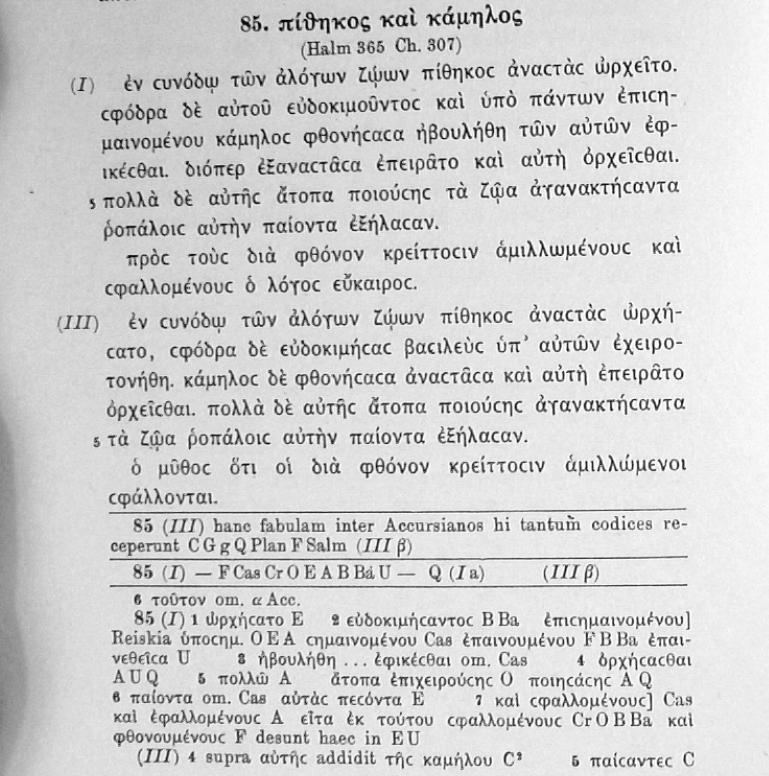
\includegraphics[width=.7\textwidth]{imgs/Edizione-Critica-apparato.png}
    \end{center}

\end{frame}



\begin{frame}
    \frametitle{TEI Modulo 12 - Codifica Edizioni Critiche}
    \framesubtitle{Getting started}
    \addtocounter{nframe}{1}

    
    % * Evidenziazione, page 1
    % Witnesses to a text may include authorial or other manuscripts, printed editions of the work, early translations, or quotations of a work in other texts


    \begin{block}{Edizioni critiche di testi}
        I documenti testimoni di un testo (\textit{tradizione}) possono essere di varia natura:
        \begin{itemize}
            \item manoscritti d'autore
            \item manoscritti copia
            \item edizioni a stampa
            \item traduzioni
            \item citazioni in testimonianze indirette
            \item ...
        \end{itemize}
    \end{block}

\end{frame}

\begin{frame}
    \frametitle{TEI Modulo 12 - Codifica Edizioni Critiche}
    \addtocounter{nframe}{1}
    
    \begin{center}
        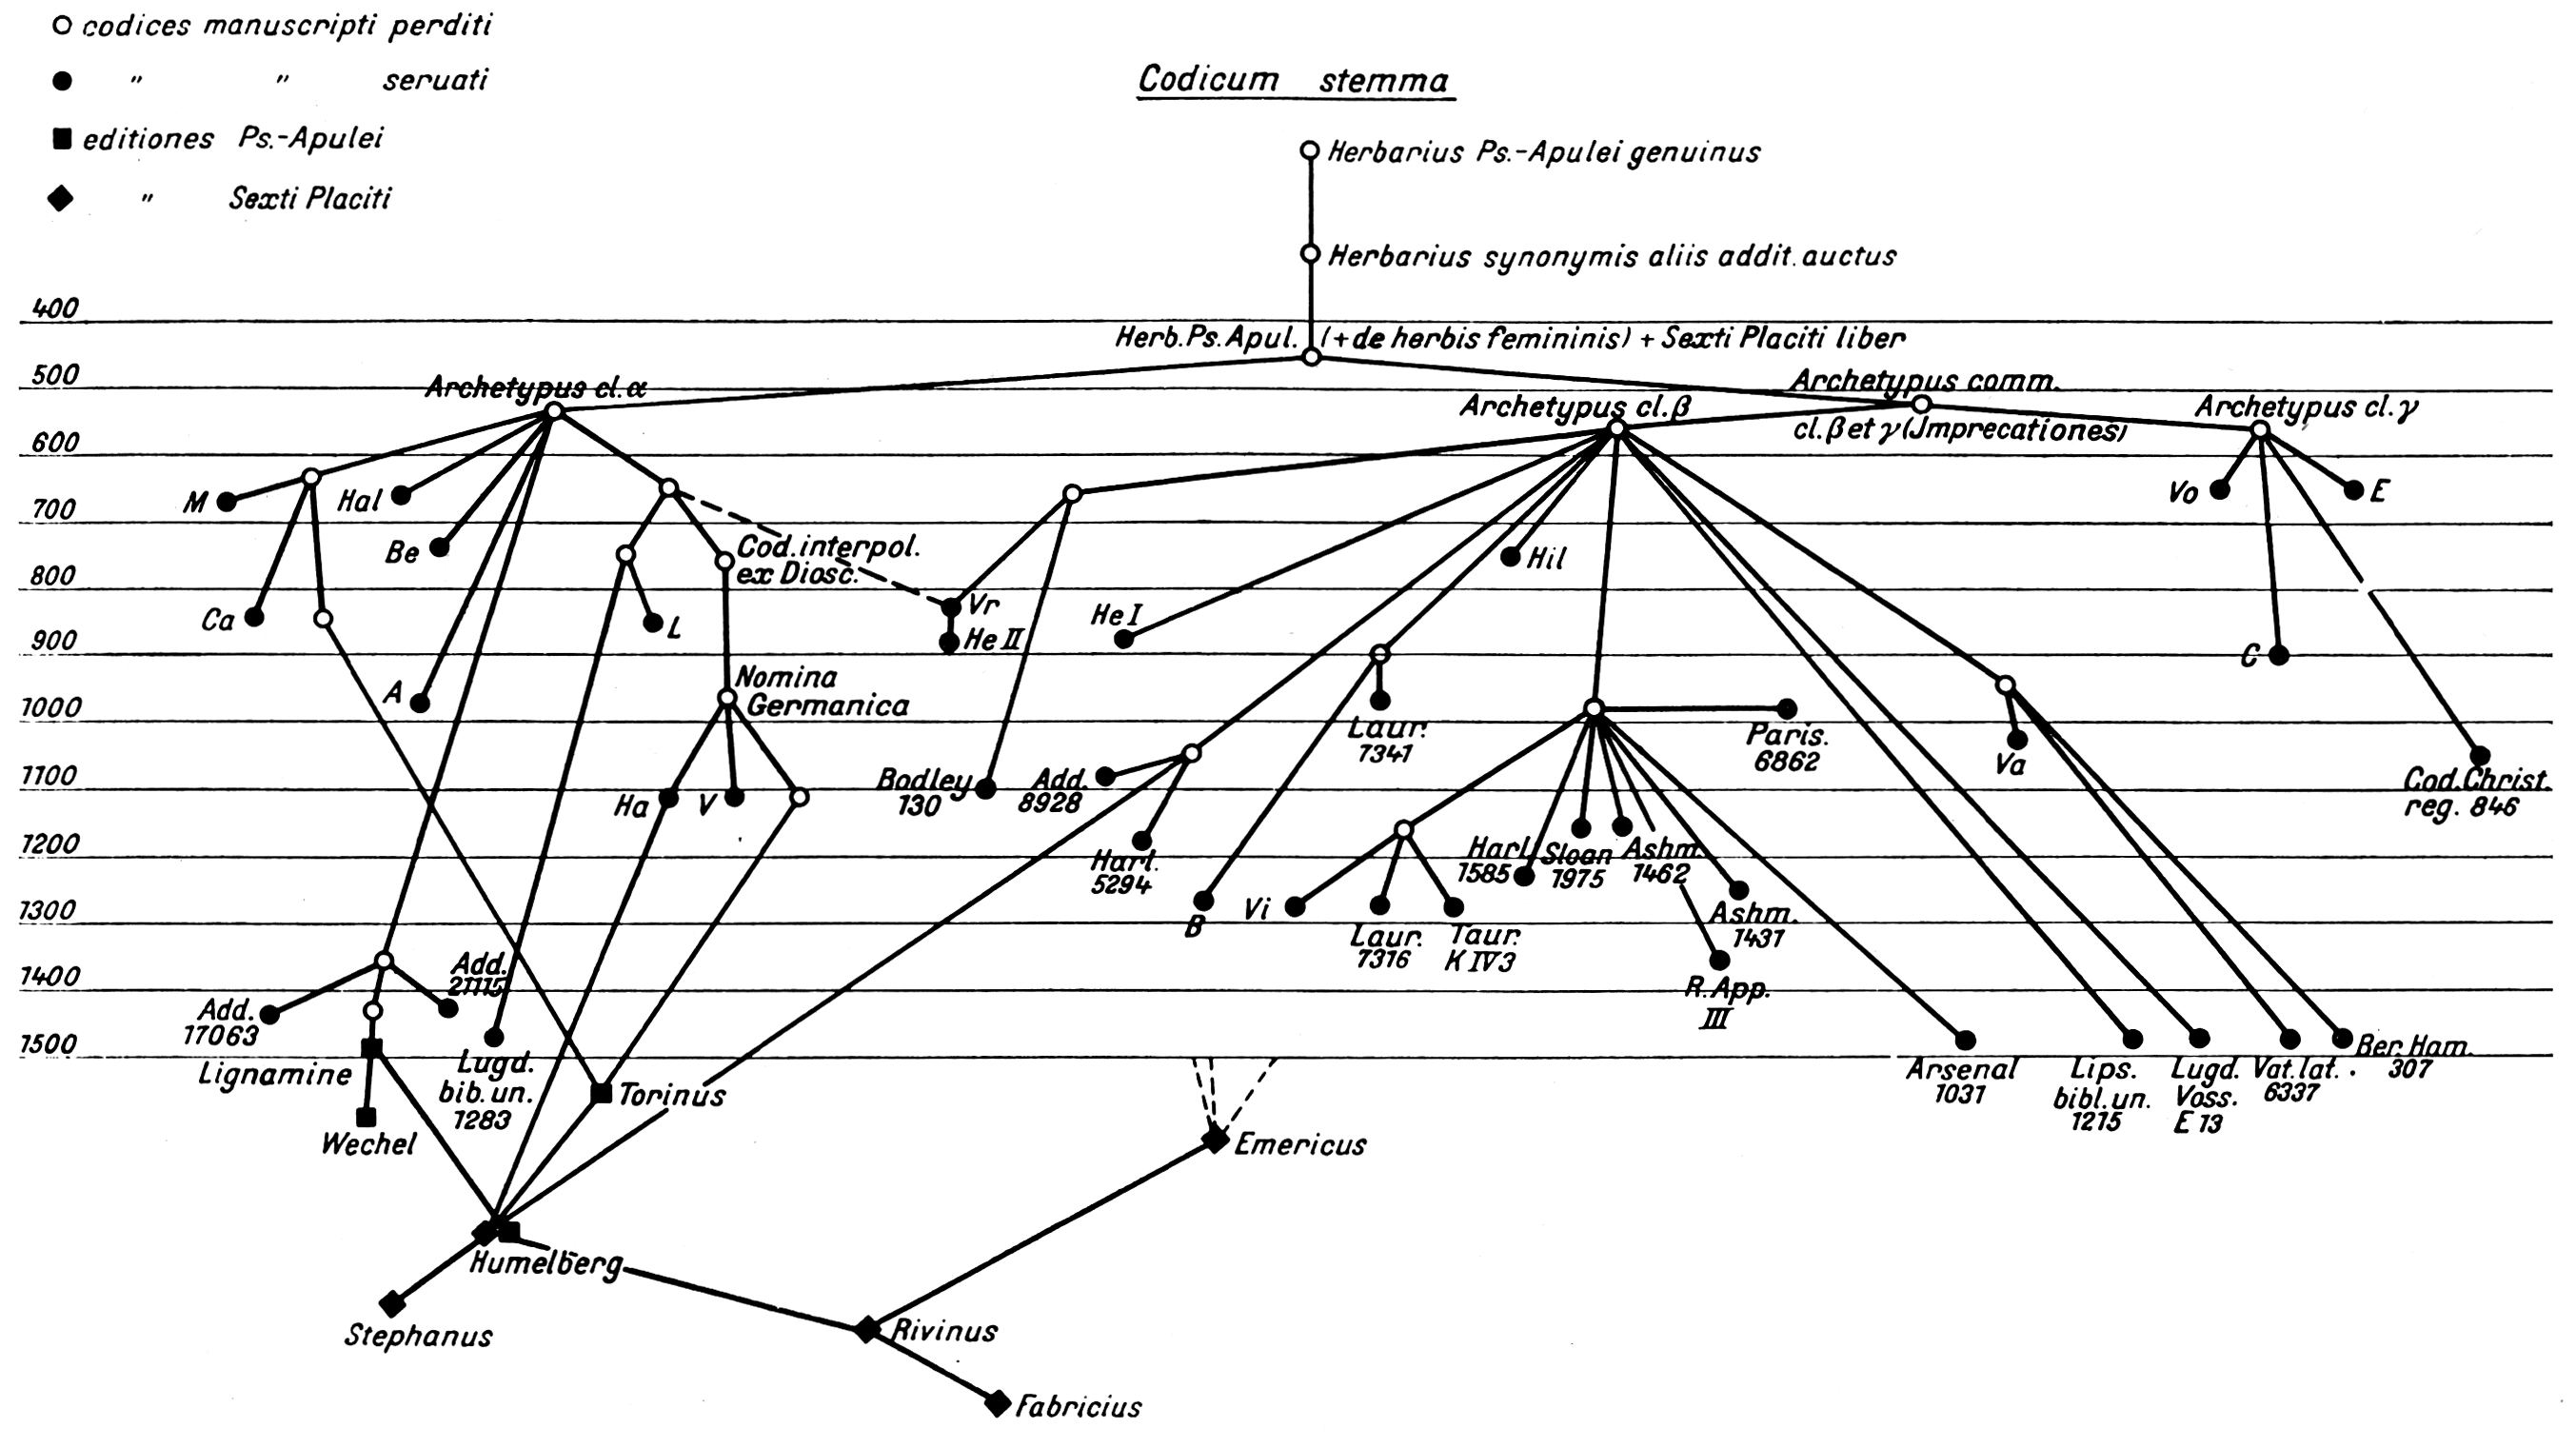
\includegraphics[width=.95\textwidth]{imgs/image.png}
    \end{center}

\end{frame}

\begin{frame}
    \frametitle{TEI Modulo 12 - Codifica Edizioni Critiche}
    \framesubtitle{Getting started}
    \addtocounter{nframe}{1}


    \begin{block}{Cosa rappresenta un apparato critico}
        \begin{itemize}
            \item Rappresentare diverse versioni di uno stesso passo di testo lette da diverse fonti
            \item Accompagnare la scelta dell'editore nel lavoro di ricostruzione del testo
            \item Rappresentare una diramazione del testo nella tradizione e un conseguente ricongiungimento
        \end{itemize}
    \end{block}
       
\end{frame}

\begin{frame}
    \frametitle{TEI Modulo 12 - Codifica Edizioni Critiche}
    \addtocounter{nframe}{1}
    
    \textbf{semplice esempio del grafo delle varianti}

    \begin{center}
        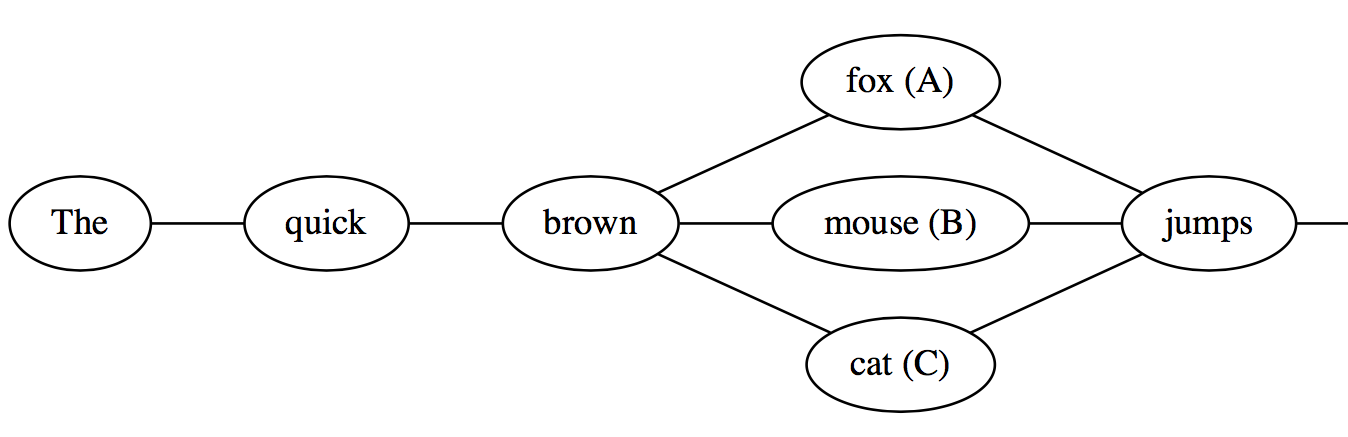
\includegraphics[width=.95\textwidth]{imgs/testo-divergente.png}
    \end{center}

    \textit{image from \url{http://doi.org/10.5281/zenodo.3446155}}

\end{frame}

\begin{frame}
    \frametitle{TEI Modulo 12 - Codifica Edizioni Critiche}
    \framesubtitle{Getting started}
    \addtocounter{nframe}{1}

    % * Evidenziazione, page 1
    % encoding such an apparatus of variants

    % * Evidenziazione, page 1
    % provides extra attributes for some elements of the core tag set when this module is selected
    
    \begin{block}{Obiettivo del modulo 12 (Critical Apparatus)}
        Codificare in forma strutturata l'apparato critico e l'insieme dei testimoni
    \end{block}

    \begin{block}{Modulo 12 delle linee guida TEI}
        Definisce elementi, attributi e prassi per la rappresentazione digitale di edizioni critiche
    \end{block}

\end{frame}

\begin{frame}
    \frametitle{TEI Modulo 12 - Codifica Edizioni Critiche}
    \framesubtitle{Getting started}
    \addtocounter{nframe}{1}

    % * Evidenziazione, page 1
% variant readings

% * Evidenziazione, page 1
% may be recorded in a series of apparatus entries

% * Evidenziazione, page 1
% documentation of the witnesses whose readings are included in the apparatus

    \begin{block}{Modulo 12 delle linee guida TEI}
       Grazie alle specifiche del modulo è possibile registrare la lezione a testo e le lezioni non accolte dei vari testimoni della tradizione
    \end{block}

    \begin{block}{Modulo 12 delle linee guida TEI}
       Documentare i dettagli dei testimoni i quali sono rappresentati con sigle distintive
     \end{block}

\end{frame}

\begin{frame}
    \frametitle{TEI Modulo 12 - Codifica Edizioni Critiche}
    \framesubtitle{Getting started}
    \addtocounter{nframe}{1}


    \begin{block}{Modulo 12 delle linee guida TEI}
        \begin{itemize}
            \item registrare contenuto di testimoni frammentari
            \item registrare le entrate di apparato intercalandole al testo principale (embedded/inline)
            \item registrare le entrate di apparato separate dal testo principale (apparato esterno)
        \end{itemize}
    \end{block}


\end{frame}

\begin{frame}
    \frametitle{TEI Modulo 12 - Codifica Edizioni Critiche}
    \framesubtitle{Apparatus, Readings, Witnesses}
    \addtocounter{nframe}{1}

    % * Evidenziazione, page 1
    % Apparatus

    % * Evidenziazione, page 1
    % Readings

    % * Evidenziazione, page 1
    % Witnesses

    % * Evidenziazione, page 1
    % fundamental markup methods used to encode textual variations

    % * Evidenziazione, page 2
    % the app element for entries in the critical apparatus

    % * Evidenziazione, page 2
    % identifying individual readings

    % * Evidenziazione, page 2
    % ways of grouping readings together

    % * Evidenziazione, page 2
    % identifying which witnesses support a particular reading

    % * Evidenziazione, page 2
    % describing the witnesses included in the apparatus

    % * Evidenziazione, page 2
    % which portions of a text are covered by fragmentary witnesses

    \begin{block}{Elementi fondamentali per la codifica di un testo critico}
        \begin{itemize}
            \item Le singole entrate di apparato sono rappresentate dall'elemento \texttt{<app>}
            \item Le differenti letture sono registrate con l'elemento \texttt{<rdg>}
            \item La lettura accolta a testo è registrata con l'elemento \texttt{<lemma>}
            \item I testimoni sono registrati con l'elemento \texttt{<witness>}
        \end{itemize}
       
    \end{block}


\end{frame}


\begin{frame}
    \frametitle{TEI Modulo 12 - Codifica Edizioni Critiche}
    \framesubtitle{Apparatus, Readings, Witnesses}
    \addtocounter{nframe}{1}

    % * Evidenziazione, page 1
    % Apparatus

    % * Evidenziazione, page 1
    % Readings

    % * Evidenziazione, page 1
    % Witnesses

    % * Evidenziazione, page 1
    % fundamental markup methods used to encode textual variations

    % * Evidenziazione, page 2
    % the app element for entries in the critical apparatus

    % * Evidenziazione, page 2
    % identifying individual readings

    % * Evidenziazione, page 2
    % ways of grouping readings together

    % * Evidenziazione, page 2
    % identifying which witnesses support a particular reading

    % * Evidenziazione, page 2
    % describing the witnesses included in the apparatus

    % * Evidenziazione, page 2
    % which portions of a text are covered by fragmentary witnesses

    \begin{block}{Elementi fondamentali per la codifica di un testo critico}
        \begin{itemize}
            \item Le varianti possono essere raggruppate con l'elemento \texttt{<rgdGrp>}
            \item La tradizione dei testimoni considerati sono raggruppati nell'elemento \texttt{<listWit>}
            \item I testimoni possono essere indicati anche accanto alla variante con l'elemento \texttt{<wit>}
        \end{itemize}
       
    \end{block}

\end{frame}

\begin{frame}
    \frametitle{TEI Modulo 12 - Codifica Edizioni Critiche}
    \framesubtitle{Apparatus, Readings, Witnesses}
    \addtocounter{nframe}{1}

    % * Evidenziazione, page 2
% The app element

% * Evidenziazione, page 2
% The individual apparatus entry is encoded with the app element

% * Evidenziazione, page 2
% a way of marking points where the encoding of a passage in a single source may be carried out in more than one way


% * Evidenziazione, page 2
% Individual textual variations are encoded using the app element

% * Evidenziazione, page 2
% which groups together all the readings constituting the variation

% * Evidenziazione, page 2
% is not a purely mechanical process

% * Evidenziazione, page 2
% Each app element usually comprises one or more readings


    \begin{block}{L'elemento \texttt{<app>}}

        TODO

    \end{block}


\end{frame}


\begin{frame}
    \frametitle{TEI Modulo 12 - Codifica Edizioni Critiche}
    \framesubtitle{Apparatus, Readings, Witnesses}
    \addtocounter{nframe}{1}

    % * Evidenziazione, page 2
% several methods may be used for such linkage

    \begin{block}{Metodi per codificare l'apparato critico}
        \begin{itemize}
            \item location-referenced method
            \item double-end-point-attached method
            \item the parallel segmentation method
        \end{itemize}

       
    \end{block}


\end{frame}


\begin{frame}
    \frametitle{TEI Modulo 12 - Codifica Edizioni Critiche}
    \framesubtitle{Apparatus, Readings, Witnesses}
    \addtocounter{nframe}{1}

    % * Evidenziazione, page 2
    % <app> (apparatus entry) contains one entry in a critical apparatus, with an optional lemma and usually one or more readings or notes on the relevant passage.

    % * Evidenziazione, page 2
    % @type

    % * Evidenziazione, page 2
    % classifies the variation contained in this element according to some convenient typology

    % * Evidenziazione, page 2
    % @from

    % * Evidenziazione, page 2
    % identifies the beginning of the lemma in the base text.

    % * Evidenziazione, page 2
    % @to

    % * Evidenziazione, page 2
    % identifies the endpoint of the lemma in the base text.

    % * Evidenziazione, page 2
    % @loc

    % * Evidenziazione, page 2
    % location

    % * Evidenziazione, page 2
    % indicates the location of the variation

    % * Evidenziazione, page 2
    % The attributes @loc, @from, and @to, are used to link the apparatus entry to the base text

    \begin{block}{L'elemento \texttt{<app>}}
        \texttt{<app>} (\textit{apparatus entry}) contains one entry in a critical apparatus, with an optional lemma and usually one or more readings or notes on the relevant passage.
    \end{block}

\end{frame}

\begin{frame}
    \frametitle{TEI Modulo 12 - Codifica Edizioni Critiche}
    \framesubtitle{Apparatus, Readings, Witnesses}
    \addtocounter{nframe}{1}

    % * Evidenziazione, page 2
    % <app> (apparatus entry) contains one entry in a critical apparatus, with an optional lemma and usually one or more readings or notes on the relevant passage.

    % * Evidenziazione, page 2
    % @type

    % * Evidenziazione, page 2
    % classifies the variation contained in this element according to some convenient typology

    % * Evidenziazione, page 2
    % @from

    % * Evidenziazione, page 2
    % identifies the beginning of the lemma in the base text.

    % * Evidenziazione, page 2
    % @to

    % * Evidenziazione, page 2
    % identifies the endpoint of the lemma in the base text.

    % * Evidenziazione, page 2
    % @loc

    % * Evidenziazione, page 2
    % location

    % * Evidenziazione, page 2
    % indicates the location of the variation

    % * Evidenziazione, page 2
    % The attributes @loc, @from, and @to, are used to link the apparatus entry to the base text

    \begin{block}{Attributi significativi dell'elemento <app>}
        \begin{itemize}
            \item \texttt{@type}: \textit{classifies the variation contained in this element according to some convenient typology}
            \item \texttt{@from}: \textit{identifies the beginning of the lemma in the base text.}
            \item \texttt{@to}: \textit{identifies the endpoint of the lemma in the base text}
            \item \texttt{@loc} \textit{indicates the location of the variation}
        \end{itemize}
    \end{block}

    \textit{Gli attributi @loc, @from, and @to, sono impiegati per collegare l'entrata di apparato al testo principale (esistono vari metodi)}


\end{frame}

\begin{frame}
    \frametitle{TEI Modulo 12 - Codifica Edizioni Critiche}
    \addtocounter{nframe}{1}
    
    % * Evidenziazione, page 2
    % A very simple partial apparatus

    % * Evidenziazione, page 3
    % in practice the apparatus will be somewhat more complex

    \begin{center}
        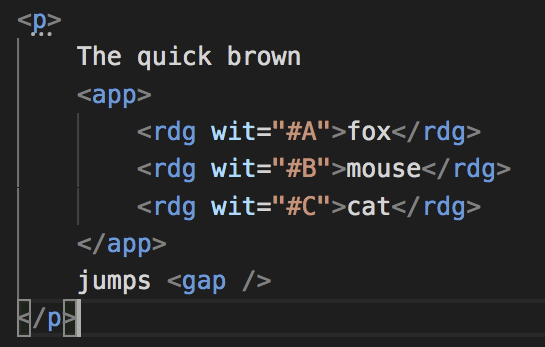
\includegraphics[width=.95\textwidth]{imgs/fox-jumps.png}
    \end{center}

\end{frame}



% * Evidenziazione, page 3
% readings

% * Evidenziazione, page 3
% subvariation

% * Evidenziazione, page 3
% witness information

% * Evidenziazione, page 3
% Individual readings are the crucial elements in any critical apparatus of variants

% * Evidenziazione, page 3
% tag individual readings within an apparatus entry:

% * Evidenziazione, page 3
% <lem>

% * Evidenziazione, page 3
% lemma

% * Evidenziazione, page 3
% contains the lemma, or base text, of a textual variation

% * Evidenziazione, page 3
% <rdg>

% * Evidenziazione, page 3
% reading

% * Evidenziazione, page 3
% contains a single reading within a textual variation.

% * Evidenziazione, page 3
% the term lemma is used here in the text-critical sense of ‘the reading accepted as that of the original or of the base text’

% * Evidenziazione, page 3
% In recording readings within an apparatus entry, the rdg element should always be used; each app usually contains at least one rdg, though it may contain only notes.

% * Evidenziazione, page 3
% The lem element may also be used to record the base text of the source edition

% * Evidenziazione, page 3
% mark the readings of a base witness, to indicate the preference of an editor or encoder for a particular reading, or (e.g. in the case of an external apparatus) to indicate precisely to which portion of the main text the variation applies.

% * Evidenziazione, page 3
% may prefer not to use it at all

% * Evidenziazione, page 3
% How it is used depends in part on the method chosen for linking the apparatus to the text

% * Evidenziazione, page 3
% Readings may be encoded individually, or grouped for perspicuity using the rdgGrp element

% * Evidenziazione, page 3
% attribute classes att.witnessed and att.textCritical,

% * Evidenziazione, page 3
% attributes

% * Evidenziazione, page 3
% attribute used to identify the witnesses supporting a particular reading in a critical apparatus.

% * Evidenziazione, page 4
% @wit

% * Evidenziazione, page 4
% witness

% * Evidenziazione, page 4
% witnesses

% * Evidenziazione, page 4
% contains a space-delimited list of one or more pointers indicating the witnesses which attest to a given reading.

% * Evidenziazione, page 4
% set of attributes common to all elements representing variant readings in text critical work

% * Evidenziazione, page 4
% type

% * Evidenziazione, page 4
% classifies the reading according to some useful typology

% * Evidenziazione, page 4
% substantive

% * Evidenziazione, page 4
% orthographic

% * Evidenziazione, page 4
% cause

% * Evidenziazione, page 4
% he cause for the variant reading

% * Evidenziazione, page 4
% homeoteleuton

% * Evidenziazione, page 4
% homeoarchy

% * Evidenziazione, page 4
% paleographicConfusion

% * Evidenziazione, page 4
% haplography

% * Evidenziazione, page 4
% dittography

% * Evidenziazione, page 4
% falseEmendation

% * Evidenziazione, page 4
% varSeq

% * Evidenziazione, page 4
% variant sequence

% * Evidenziazione, page 4
% number indicating the position of this reading in a sequence

% * Evidenziazione, page 4
% hand

% * Evidenziazione, page 4
% points to a handNote element describing the hand considered responsible

% * Evidenziazione, page 4
% att.written

% * Evidenziazione, page 4
% nherit the following attributes from the att.global.responsibility class

% * Evidenziazione, page 4
% attributes indicating the agent responsible for some aspect of the text

% * Evidenziazione, page 4
% resp

% * Evidenziazione, page 4
% esponsible party

% * Evidenziazione, page 4
% agency responsible for the intervention or interpretation, for example an editor or transcriber

% * Evidenziazione, page 4
% cert

% * Evidenziazione, page 4
% certainty

% * Evidenziazione, page 4
% the degree of certainty associated with the intervention or interpretation

% * Evidenziazione, page 4
% these attributes may be used to indicate the person responsible for the editorial decision being recorded

% * Evidenziazione, page 4
% also the degree of certainty associated with that decision by the person carrying out the encoding

% * Evidenziazione, page 4
% The @wit attribute identifies the witnesses which have the reading in question

% * Evidenziazione, page 4
% It is required if the apparatus gathers together readings from different witnesses

% * Evidenziazione, page 4
% The @type attribute allows the encoder to classify readings in any convenient way

% * Evidenziazione, page 4
% substantive variants of the lemma

% * Evidenziazione, page 5
% substantive

% * Evidenziazione, page 5
% or as orthographic variants:

% * Evidenziazione, page 5
% The @varSeq and @cause attributes may be used to convey information on the sequence and cause of variation.

% * Evidenziazione, page 5
% the reading Eryment is tagged as sequential to (derived from) the reading Experiment, and the cause is given as loss of the abbreviation for per.

% * Evidenziazione, page 5
% <app> <rdg wit="#La" varSeq="1">Experiment</rdg> <rdg wit="#Ra2" cause="abbreviation_loss" varSeq="2">Eryment</rdg> </app>

% * Evidenziazione, page 5
% cause

% * Evidenziazione, page 5
% If a manuscript is written in several hands, and it is desired to report which hand wrote a particular reading, the @hand attribute should be used.

% * Evidenziazione, page 5
% in the Munich manuscript containing the Carmina Burana, the word alle has been changed to allen:

% * Evidenziazione, page 5
% <app> <rdg wit="#Mu" varSeq="1" hand="#m1">alle</rdg> <rdg wit="#Mu" cause="nachgetragen" varSeq="2" hand="#m2">allen</rdg> </app>

% * Evidenziazione, page 5
% Similarly, if a witness is hard to decipher, it may be desired to indicate responsibility for the claim that a particular reading is supported by a particular witness.

% * Evidenziazione, page 5
% the manuscript is read in different ways by different scholars

% * Evidenziazione, page 5
% records in the apparatus two different accounts of the manuscript reading

% * Evidenziazione, page 5
% <rdg wit="#ms" source="#Z">heaðo hlæwe</rdg> <rdg wit="#ms" source="#Cha">heaum hope</rdg>

% * Evidenziazione, page 6
% @hand attribute indicates a particular manuscript hand

% * Evidenziazione, page 6
% Where there is a greater weight of editorial discussion and interpretation

% * Evidenziazione, page 6
% this information can be attached to the apparatus in a note.

% * Evidenziazione, page 6
% The note element may also be used to record the specific wording of notes in the apparatus of the source edition

% * Evidenziazione, page 6
% <note source="#Kl">

% * Evidenziazione, page 6
% Notes providing details of the reading of one particular witness should be encoded using the specialized witDetail element

% * Evidenziazione, page 6
% Encoders should be aware of the distinct fields of use of the attribute values @wit, @hand, and @source

% * Evidenziazione, page 6
% @wit identifies the physical entity in which the reading is found (manuscript, clay tablet, papyrus, printed edition);

% * Evidenziazione, page 6
% @hand refers to the agent responsible for inscribing that reading in that physical entity (scribe, author, inscriber, hand 1, hand 2)

% * Evidenziazione, page 6
% @source indicates the scholar responsible for asserting the existence of that reading in that physical entity

% * Evidenziazione, page 6
% the categories may blur: a scholar may produce an edition introducing readings for which he or she is responsible; that edition may itself become a witness in a later critical apparatus.

% * Evidenziazione, page 6
% Subvariation

% * Evidenziazione, page 6
% The rdgGrp element may be used to group readings

% * Evidenziazione, page 6
% they have identical values on one or more attributes, or because they are seen as forming a self-contained variant sequence, or for some other reason

% * Evidenziazione, page 7
% <rdgGrp>

% * Evidenziazione, page 7
% reading group

% * Evidenziazione, page 7
% groups two or more readings perceived to have a genetic relationship or other affinity

% * Evidenziazione, page 7
% The rdgGrp element is a member of class att.textCritical and therefore can carry the @wit, @type, @cause, @varSeq, @hand, and @resp attributes described in the preceding section.

% * Evidenziazione, page 7
% When values for any of these attributes are given on a rdgGrp element, the values given are inherited by the rdg or lem elements nested within the reading group

% * Evidenziazione, page 7
% To indicate that both Hg and La vary only orthographically from the lemma, one might tag both readings <rdg type='orthographic'>

% * Evidenziazione, page 7
% This fact can be expressed more perspicuously, however, by grouping their readings into a rdgGrp

% * Evidenziazione, page 7
% <app> <lem wit="#El #Ra2">though</lem> <rdgGrp type="orthographic"> <rdg wit="#La">thogh</rdg> <rdg wit="#Hg">thouh</rdg> </rdgGrp> </app>

% * Evidenziazione, page 7
% Similarly, rdgGrp may be used to organize the substantive variants of an apparatus entry.

% * Evidenziazione, page 7
% Editors may need to indicate that each of a group of witnesses may be taken as all supporting a particular reading

% * Evidenziazione, page 7
% manuscripts display many different spellings of these words

% * Evidenziazione, page 7
% all these variant spellings and that these variant spellings actually support only the three regularized spelling forms

% * Evidenziazione, page 7
% One may term these variant spellings as ‘subvariants’ of the regularized spelling forms.

% * Evidenziazione, page 7
% This subvariation can be expressed within an app element by gathering the readings into three groups according to the normalized form of their reading.

% * Evidenziazione, page 7
% All the readings within each group may be accounted subvariants of the main reading for the group

% * Evidenziazione, page 7
% tagging it as a lem element or as <rdg type='groupBase'>

% * Evidenziazione, page 7
% In this example, the different subvariants on Experience, Experiment, and Eriment are held within three rdgGrp elements nested within the enclosing app element:

% * Evidenziazione, page 7
% <app type="substantive"> <rdgGrp type="subvariants"> <lem wit="#El #Hg">Experience</lem> <rdg wit="#Ha4">Experiens</rdg> </rdgGrp> <rdgGrp type="subvariants"> <lem wit="#Cp #Ld1">Experiment</lem> <rdg wit="#La">Ex<g ref="#per"/>iment</rdg> </rdgGrp> <rdgGrp type="subvariants"> <lem resp="#ed2013">Eriment</lem>

% * Evidenziazione, page 8
% <rdg wit="#Ra2">Eryment</rdg> </rdgGrp> </app>

% * Evidenziazione, page 8
% From this, one may deduce that the regularized reading Experience is supported by all three manuscripts El Hg Ha4, although the spelling differs in Ha4, and that the regularized reading Eriment is supported by Ra2, even though the form differs in that manuscript.

% * Evidenziazione, page 8
% Thus, Ha4 here supports the reading Experience found in El and Hg, even though it is spelt slightly differently in Ha4.

% * Evidenziazione, page 8
% Reading groups may nest recursively, so that variants can be classified to any desired depth.

% * Evidenziazione, page 8
% Because apparatus entries may also nest, the app element might also be used to group readings in the same way.

% * Evidenziazione, page 8
% <app n="a1" type="substantive"> <rdg wit="#El #Hg #Ha4"> <app n="a2" type="orthographic"> <lem wit="#El #Hg">Experience</lem> <rdg wit="#Ha4">Experiens</rdg> </app> </rdg> <rdg wit="#Cp #Ld1 #La"> <app n="a3" type="orthographic"> <lem wit="#Cp #Ld1">Experiment</lem> <rdg wit="#La">Ex<g ref="#per"/>iment</rdg> </app> </rdg> <rdg wit="#Ra2"> <app n="a4" type="orthographic"> <lem resp="#ed2013">Eriment</lem> <rdg wit="#Ra2">Eryment</rdg> </app> </rdg> </app>

% * Evidenziazione, page 8
% this variation has three normalized readings, and that the first of these is supported by manuscripts El, Hg, and Ha4; the second by Cp, Ld1, and La; and the third by Ra2

% * Evidenziazione, page 8
% Reading groups may also be used to bring together variants which form an apparent developmental sequence

% * Evidenziazione, page 9
% <rdgGrp type="sequence"> <rdgGrp varSeq="1" type="subvariants"> <lem wit="#Cp #Ld1">Experiment</lem> <rdg wit="#La">Ex<g ref="#per"/>iment</rdg> </rdgGrp> <rdgGrp varSeq="2" cause="abbreviation_loss"> <lem resp="#ed2013">Eriment</lem> <rdg wit="#Ra2">Eryment</rdg> </rdgGrp> </rdgGrp> </app>

% * Evidenziazione, page 9
% A given reading is associated with the set of witnesses attesting it by listing the witnesses in the @wit attribute on the rdg or lem element

% * Evidenziazione, page 9
% associate annotation on a reading with one specific witness among several

% * Evidenziazione, page 9
% ranscribe witness information verbatim from a source edition

% * Evidenziazione, page 9
% identify the formal lists of witnesses typically provided in the front matter of critical editions

% * Evidenziazione, page 9
% give additional information about the reading of a particular witness or witnesses

% * Evidenziazione, page 9
% that information may be given in a witDetail element

% * Evidenziazione, page 9
% can be linked to both a reading and to one or more of the witnesses for that reading

% * Evidenziazione, page 9
% The link to the reading

% * Evidenziazione, page 9
% made explicit by the @target attribute

% * Evidenziazione, page 9
% the link to the witness, by the @wit attribute

% * Evidenziazione, page 9
% @target specifies the destination of the reference

% * Evidenziazione, page 9
% <witDetail> (witness detail) gives further information about a particular witness, or witnesses, to a particular reading

% * Evidenziazione, page 9
% @wit (witnesses) indicates the sigil or sigla identifying the witness or witnesses to which the detail refers

% * Evidenziazione, page 9
% he witDetail refers to multiple readings, @target must be used to point to the reading(s) being annotated

% * Evidenziazione, page 10
% <app type="substantive"> <lem wit="#El #Hg">Experience</lem> <witDetail wit="#El">Ornamental capital.</witDetail> <rdg wit="#Ha4">Experiens</rdg> </app>

% * Evidenziazione, page 10
% may be used to record the specific wording of information in the source text

% * Evidenziazione, page 10
% to record the wording of the note explaining that the variant reading adds n to the original in a second hand:

% * Evidenziazione, page 10
% <l> <app> <rdg wit="#Mu" hand="#m1">alle</rdg> <rdg wit="#Mu" hand="#m2">allen</rdg> <witDetail wit="#Mu"> <mentioned>n</mentioned> nachgetragen. </witDetail> </app> disen sumer gân. </l>

% * Nota ancorata, page 10
% nota sigla 

% The Latin word siglum (sign), pl. sigla denotes the abbreviation used in a critical apparatus to indicate a particular witness

% * Evidenziazione, page 10
% lists of sigla

% * Evidenziazione, page 10
% may be complex enough

% * Evidenziazione, page 10
% in the transcription of printed critical editions, it may be desirable to retain for future reference the exact form in which the source edition records the witnesses to a particular reading;

% * Evidenziazione, page 10
% The wit element may be used to transcribe such lists of witnesses to a particular reading.

% * Evidenziazione, page 10
% <wit> contains a list of one or more sigla of witnesses attesting a given reading, in a textual variation.

% * Evidenziazione, page 10
% The wit list may appear following a rdg, rdgGrp, or lem element in any apparatus entry

% * Evidenziazione, page 10
% wit may be used in a way functionally equivalent to @wit if the sigla therein are wrapped in refs with @target attributes pointing to a predefined witness

% * Evidenziazione, page 11
% <app> <lem>Nondum</lem> <rdg wit="#G #P" ana="#orthographical">nundum</rdg> <wit> <ref target="#G">G</ref>(corr. <ref target="#G1">G<hi rend="super">1</hi> </ref>)<ref target="#P">P</ref> </wit> </app>

% * Evidenziazione, page 11
% @wit is more succinct,

% * Evidenziazione, page 11
% using @wit (with witDetail when needed) is almost always to be preferred

% * Evidenziazione, page 11
% A list of all identified witnesses should normally be supplied in the front matter of the edition, or in the sourceDesc element of its header

% * Evidenziazione, page 11
% may be given either as a simple bibliographic list

% * Evidenziazione, page 11
% or as a listWit element,

% * Evidenziazione, page 11
% which contains a series of witness elements

% * Evidenziazione, page 11
% Each witness element may contain a brief characterization of the witness, given as one or more prose paragraphs

% * Evidenziazione, page 11
% nformation about a manuscript witness is available, it should be represented using the msDesc element provided by the msdescription module; a msDesc may appear within a listBibl.

% * Evidenziazione, page 11
% a unique siglum for this source should always be supplied,

% * Evidenziazione, page 11
% This identifier can then be used elsewhere to refer to this particular witness

% * Evidenziazione, page 11
% <listWit> (witness list) lists definitions for all the witnesses referred to by a critical apparatus, optionally grouped hierarchically.

% * Evidenziazione, page 11
% <witness> contains either a description of a single witness referred to within the critical apparatus, or a list of witnesses which is to be referred to by a single sigil.

% * Evidenziazione, page 11
% <msDesc> (manuscript description) contains a description of a single identifiable manuscript or other text-bearing object such as early printed books.

% * Evidenziazione, page 11
% <bibl> (bibliographic citation) contains a loosely-structured bibliographic citation of which the sub-components may or may not be explicitly tagged.

% * Evidenziazione, page 11
% <listBibl> (citation list) contains a list of bibliographic citations of any kind.

% * Evidenziazione, page 12
% witness list is thus the set of sigla for all the witnesses named in the apparatus

% * Evidenziazione, page 12
% <listWit> <witness xml:id="Chi3"/> <witness xml:id="Ha4"/> <witness xml:id="Ju"/> <witness xml:id="K"/> <witness xml:id="Kb"/> <witness xml:id="Kl"/> <witness xml:id="Kv"/> <witness xml:id="Ld"/> <witness xml:id="Ld1"/> <witness xml:id="Ln"/> <witness xml:id="Mu"/> <witness xml:id="Ry2"/> <witness xml:id="Wa"/> <witness xml:id="X"/> </listWit>

% * Evidenziazione, page 12
% each witness element should contain at least a brief prose description of the witness

% * Evidenziazione, page 12
% including a bibliographic citation

% * Evidenziazione, page 12
% <witness xml:id="Ra2">Bodleian Library Rawlinson Poetic 149 (see further <ptr target="http://example.com/msDescs#MSRP149"/>)</witness>

% * Evidenziazione, page 12
% the witness description here may be complemented by a reference to a full description of the manuscript supplied elsewhere, typically as the content of a msDesc or bibl element

% * Evidenziazione, page 12
% a whole paragraph of commentary for each witnes

% * Evidenziazione, page 12
% <witness xml:id="a">Bezeichnung <bibl> <author>Lachmann</author> </bibl>s für die von einer 2. Hand auf bl. 40–43 geschriebenen Strophen der Hs. A.</witness>

% * Evidenziazione, page 13
% It would however generally be preferable to represent such detailed information using an appropriately structured msDesc element

% * Evidenziazione, page 13
% f the witnesses being recorded are not manuscripts but printed works, it may be preferable to document them using the standard bibl or biblStruct elements

% * Evidenziazione, page 13
% In text-critical work it is customary to refer to frequently occurring groups of witnesses by means of a single common siglum

% * Evidenziazione, page 13
% ncluding a nested witness list within the witness list

% * Evidenziazione, page 13
% uses the siglum for the group as its identifier

% * Evidenziazione, page 13
% supplies a fuller name for the group in its optional child head element

% * Evidenziazione, page 13
% listWit> <witness xml:id="Ellesmere">Ellesmere, Huntingdon Library 26.C.9</witness> <!-- ... --> <listWit xml:id="Con"> <head>Constant Group C</head> <witness xml:id="Cp">Corpus Christi Oxford MS 198</witness> <witness xml:id="La">British Library Lansdowne 851</witness> <witness xml:id="Sl2">British Library Sloane MS 1686</witness> </listWit> </listWit>

% * Evidenziazione, page 13
% <rdg wit="#Con">Experiment</rdg>

% * Evidenziazione, page 13
% The more elaborate example below shows both multiple levels of nesting and a strategy for mapping the the @xml:id of the witness to the siglum which will be displayed to the reader of a derived visualisation

% * Evidenziazione, page 13
% <witness xml:id="Σ">Servius (<abbr type="siglum">Σ</abbr>) = ΔΓ

% * Evidenziazione, page 13
% <witness xml:id="Δ">

% * Evidenziazione, page 14
% <abbr type="siglum">Δ</abbr>

% * Evidenziazione, page 14
% <witness xml:id="Γ">

% * Evidenziazione, page 14
% <abbr type="siglum">Γ</abbr>

% * Evidenziazione, page 15
% Here we have a summary of the witnesses, with their sigla, used in an edition, as is generally found in the conspectus siglorum in the front matter of a critical edition.

% * Evidenziazione, page 15
% Families are indicated with Greek letters and manuscript witnesses with Latin letters

% * Evidenziazione, page 15
% The siglum for display is always contained in the abbr with @type ‘siglum’

% * Evidenziazione, page 15
% Situations commonly arise where there are many more or less fragmentary witnesses

% * Evidenziazione, page 15
% there may be quite distinct groups of witnesses for different parts of a text or collection of texts

% * Evidenziazione, page 15
% If a witness list is provided, it may be unnecessary to give, in each apparatus entry, an exhaustive list of the witnesses which agree with the base text

% * Evidenziazione, page 15
% hence calculate all the manuscripts agreeing with the base text

% * Evidenziazione, page 15
% encoders may find it less error-prone to list all witnesses explicitly in each apparatus entry

% * Evidenziazione, page 15
% If a witness is incomplete

% * Evidenziazione, page 15
% record explicitly where its preserved portions begin and end

% * Evidenziazione, page 15
% tags, which may occur within any lem or rdg element

% * Evidenziazione, page 15
% beginning or end of a fragmentary witness or of a lacuna

% * Evidenziazione, page 15
% <witStart> (fragmented witness start) indicates the beginning, or resumption, of the text of a fragmentary witness.

% * Evidenziazione, page 15
% <witEnd> (fragmented witness end) indicates the end, or suspension, of the text of a fragmentary witness.

% * Evidenziazione, page 16
% <lacunaStart> indicates the beginning of a lacuna in the text of a mostly complete textual witness.

% * Evidenziazione, page 16
% <lacunaEnd> indicates the end of a lacuna in a mostly complete textual witness.

% * Evidenziazione, page 16
% In an apparatus this might appear thus, distinguished from the reading of other manuscripts by the presence of the lacunaEnd element:

% * Evidenziazione, page 16
% <app> <lem wit="#El #Hg">Auctoritee</lem> <rdg wit="#La #Ra2">auctorite</rdg> <rdg wit="#X"> <lacunaEnd/>auctorite</rdg> </app>

% * Evidenziazione, page 16
% <app> <lem wit="#El #Hg">Auctoritee</lem> <rdg wit="#La #Ra2 #X"> <lacunaEnd wit="#X"/>auctorite</rdg> </app>

% * Evidenziazione, page 16
% In some cases, the apparatus in the source may commence recording the readings for a particular witness without its being clear whether the previous absence of readings for this witness is due to a lacuna

% * Evidenziazione, page 16
% The witStart element may be used in this circumstance:

% * Evidenziazione, page 16
% <app> <lem wit="#El #Hg">Auctoritee</lem> <rdg wit="#La #Ra2">auctorite</rdg> <rdg wit="#X"> <witStart/>auctorite</rdg> </app>

% * Evidenziazione, page 16
% Three different methods may be used to link a critical apparatus to the text:

% * Evidenziazione, page 16
% the location-referenced method,

% * Evidenziazione, page 16
% the double-end-point-attached method

% * Evidenziazione, page 16
% the parallel segmentation method

% * Evidenziazione, page 16
% the location-referenced and the double end-point methods may be used with either in-line or external apparatus

% * Evidenziazione, page 16
% former dispersed within the base text

% * Evidenziazione, page 16
% latter held in some separate

% * Nota ancorata, page 16
% Ci si riferisce al metodo inline

% Ci si riferisce al metodo inline

% * Evidenziazione, page 17
% location

% * Evidenziazione, page 17
% within or outside the document with the base text

% * Evidenziazione, page 17
% The parallel segmentation method does not use the concept of a base text and may only be used for in-line apparatus

% * Evidenziazione, page 17
% Where an external apparatus is used, the listApp element provides a useful means of grouping together a series of app elements of a specific type, or from a particular source

% * Evidenziazione, page 17
% <listApp>

% * Evidenziazione, page 17
% ist of apparatus entries.

% * Evidenziazione, page 17
% attributes which can be used to classify or subclassify elements

% * Evidenziazione, page 17
% @type

% * Evidenziazione, page 17
% @subtype

% * Evidenziazione, page 17
% listApp elements would normally appear in the back of a document, but they may also be placed in any other convenient location.

% * Evidenziazione, page 17
% Any document containing app elements requires a variantEncoding declaration in the encodingDesc element of its TEI heade

% * Evidenziazione, page 17
% <variantEncoding> declares the method used to encode text-critical variants.

% * Evidenziazione, page 17
% @method

% * Evidenziazione, page 17
% @location

% * Evidenziazione, page 17
% appears within the running text or external

% * Evidenziazione, page 17
% The location-referenced method of encoding apparatus provides a convenient method for encoding printed apparatus

% * Evidenziazione, page 17
% the apparatus is linked to the base text by indicating explicitly only the block of text on which there is a variant

% * Evidenziazione, page 17
% usually by a canonical reference scheme, or by line number in the edition

% * Evidenziazione, page 17
% If the location-referenced method is used for an apparatus stored externally to the base text, the TEI header must have the declaration

% * Evidenziazione, page 17
% <variantEncoding method="location-referenced" location="external"/>

% * Evidenziazione, page 17
% In the body of the document, the base text (here El) will appear

% * Evidenziazione, page 18
% Elsewhere in the document, or in a separate file, the apparatus will appear

% * Evidenziazione, page 18
% On each app element, the @loc attribute should be specified to indicate where the variant occurs in the base text.

% * Evidenziazione, page 18
% <app loc="WBP 1"> <rdg wit="#La">Experiment</rdg> <rdg wit="#Ra2">Eryment</rdg> </app>

% * Evidenziazione, page 18
% encoded using in-line storage

% * Evidenziazione, page 18
% apparatus is dispersed through the base text block to which it refers

% * Evidenziazione, page 18
% In this case, the location of the variant can be read from the line in which it occurs

% * Evidenziazione, page 18
% <variantEncoding method="location-referenced" location="internal"/>

% * Nota ancorata, page 18
% in-line location referenced method

% Quando si registrano le varianti inline, il testo base va riportato fuori dall'apparato

% * Evidenziazione, page 18
% Since the location is not required to be exact, the apparatus for a line might also appear at the end of the line:

% * Evidenziazione, page 18
% <l n="1">Experience though noon Auctoritee <app> <rdg wit="#La"> Experiment</rdg> <rdg wit="#Ra2"> Eryment</rdg> </app> </l>

% * Evidenziazione, page 18
% it is not possible to find automatically the precise portion of text varied by the readings

% * Evidenziazione, page 18
% In order to show explicitly what portion of the base text is replaced by the variant readings, the lem element may be used:

% * Evidenziazione, page 19
% no recommendations are made for conventions of abbreviating the lemma

% * Evidenziazione, page 19
% simple location-reference methods are unlikely to be as successful as the other two methods, which allow the unambiguous reconstruction of the lemma from the encoding.

% * Evidenziazione, page 19
% In the double end-point attachment method, the beginning and end of the lemma in the base text are both explicitly indicated

% * Evidenziazione, page 19
% Double end-point attachment permits unambiguous matching of each variant reading against its lemma

% * Evidenziazione, page 19
% where the apparatus is intended to enable full reconstruction of the text

% * Evidenziazione, page 19
% the @from and @to attributes of the app element are used to indicate the beginning and ending points of the reading in the base text:

% * Evidenziazione, page 19
% identifiers which occur at the locations in question

% * Evidenziazione, page 19
% If no other markup is present there, the beginning and ending points should be marked using the anchor element

% * Evidenziazione, page 19
% he beginning and end of the lemma may be indicated by using the ‘indirect pointing’ mechanisms

% * Evidenziazione, page 19
% The double end-point attachment method may be used with in-line or external apparatus

% * Evidenziazione, page 19
% the base text (here El) will appear with anchor elements inserted at every place where a variant begins or ends

% * Evidenziazione, page 19
% unless some element with an identifier already begins or ends at that point

% * Evidenziazione, page 19
% <variantEncoding method="double-end-point" location="external"/> <!-- ... --> <div n="WBP" type="prologue"> <head>The Prologe ... </head> <l n="1" xml:id="WBP.1">Experience<anchor xml:id="WBP-A2"/> though noon Auctoritee</l> <l>Were in this world ...</l> </div>

% * Evidenziazione, page 19
% separately encoded

% * Evidenziazione, page 19
% <app from="#WBP.1" to="#WBP-A2"> <rdg wit="#La">Experiment</rdg>

% * Evidenziazione, page 20
% <rdg wit="#Ra2">Eryment</rdg> </app>

% * Evidenziazione, page 20
% No anchor element is needed at the beginning of the line, since the @from attribute can use the identifier for the line as a whole

% * Evidenziazione, page 20
% the lemma is assumed to run from the beginning of the element indicated by the @from attribute, to the end of that indicated by the @to attribute

% * Evidenziazione, page 20
% If no value is given for @to, the lemma runs from the beginning to the end of the element indicated by the @from attribute.

% * Evidenziazione, page 20
% When the apparatus is encoded in-line, it is dispersed through the base text

% * Evidenziazione, page 20
% Only the beginning of the lemma need be marked with an anchor, since the app is inserted at the end of the lemma, and itself therefore marks the end of the lemma.

% * Evidenziazione, page 20
% <variantEncoding method="double-end-point" location="internal"/> <!-- ... --> <l n="1" xml:id="wbp.1">Experience <app from="#wbp.1"> <rdg wit="#La">Experiment</rdg> <rdg wit="#Ra2">Eryment</rdg> </app> though noon Auctoritee</l> <l>Were in this world ...</l>

% * Evidenziazione, page 20
% The lemma need not be repeated within the app element in this method, as it may be extracted reliably from the base text

% * Evidenziazione, page 20
% if it is desired to make an explicit record of the attestation of the base text, the lem element may be embedded within app, carrying the witnesses to the base

% * Evidenziazione, page 20
% <app from="#WBP.1" to="#WBP-A2"> <lem wit="#El #Hg">Experience</lem>

% * Evidenziazione, page 20
% This method is designed to cope with ‘overlapping lemmata’

% * Evidenziazione, page 21
% This method can readily cope with such difficult situations

% * Evidenziazione, page 21
% typically found in large and complex traditions

% * Evidenziazione, page 21
% <l xml:id="WBP.117" n="117"> And <anchor xml:id="WBP-A117.1"/> of so parfit <anchor xml:id="WBP-A117.2"/> wys <anchor xml:id="WBP-A117.3"/> a wight <anchor xml:id="WBP-A117.4"/> ywroght

% * Evidenziazione, page 21
% <app from="#WBP-A117.1" to="#WBP-A117.3"> <lem wit="#Hg">of so parfit wys</lem> <rdg wit="#Ha4">in what wise was</rdg> </app>

% * Evidenziazione, page 21
% <app from="#WBP-A117.2" to="#WBP-A117.4"> <lem wit="#Hg">wys a wight</lem> <rdg wit="#El #Ha4">was a wight</rdg> </app>

% * Evidenziazione, page 21
% The parallel segmentation method, to be discussed next, cannot handle overlaps among variants

% * Evidenziazione, page 21
% This method differs from the double end-point attachment method in that all variants at any point of the text are expressed as variants on one another.

% * Evidenziazione, page 21
% In this method, no two variations can overlap, although they may nest

% * Evidenziazione, page 21
% The texts compared are divided into matching segments all synchronized with one another

% * Evidenziazione, page 21
% It is also very easy with this method for an application to extract the full text of any one witness from the apparatus

% * Evidenziazione, page 21
% It will however be less convenient for very complex traditions

% * Evidenziazione, page 21
% In the parallel segmentation method, each segment of text on which there is variation is marked by an app element

% * Evidenziazione, page 21
% If there is a preferred (or base) reading it is tagged with lem; each reading is given in a rdg element:

% * Evidenziazione, page 22
% This method cannot be used with external apparatus

% * Evidenziazione, page 22
% it must be used in-line

% * Evidenziazione, page 22
% the witnesses to the reading most widely attested need not be stated

% * Evidenziazione, page 22
% read a listWit declaring all the witnesses to the text and then calculate which witnesses have not been named

% * Evidenziazione, page 22
% To avoid confusion, however, witnesses may be omitted only for a single reading.

% * Evidenziazione, page 22
% <l n="1"> <app> <lem>Experience</lem> <rdg wit="#La">Experiment</rdg> <rdg wit="#Ra2">Eryment</rdg> </app> though noon Auctoritee </l>

% * Evidenziazione, page 22
% apparatus entries may nest in this method

% * Evidenziazione, page 22
% the variation on the individual words of the line would nest within that for the line as a whole:

% * Evidenziazione, page 22
% <rdg wit="#Chi3">Auctoritee, though none experience</rdg> <rdg> <app> <rdg wit="#El #Hg">Experience</rdg> <rdg wit="#La">Experiment</rdg> <rdg wit="#Ra2">Eryment</rdg> </app> <app> <rdg wit="#El #Ra2">though</rdg> <rdg wit="#Hg">thogh</rdg> <rdg wit="#La">thouh</rdg> </app> <app> <rdg wit="#El #Hg">noon Auctorite</rdg> <rdg wit="#La #Ra2">none auctorite</rdg> </app> </rdg>

% * Evidenziazione, page 23
% Parallel segmentation cannot, however, deal very gracefully with variants which overlap without nesting

% * Evidenziazione, page 23
% When an apparatus is provided it does not need to be given at the location in the transcription where the variation, emendation, attribution, or other apparatus observation occurs. Instead it may be stored in a separate place in the same file, or indeed in another file, and point to the location at which it is meant to be used

% * Evidenziazione, page 23
% The location-referenced method can be used to point a position in a text using the @loc attribute and a canonical reference that is understood and documented in the context of the file where it is used

% * Evidenziazione, page 23
% Where possible it is recommended that other methods use the @from attribute to point to an @xml:id attribute on an anchor or other element at the location where the apparatus observation takes place

% * Evidenziazione, page 23
% The contents of an element pointed to are understood to be equivalent to a lem if none exists in the app, and if a lem does exist this should replace any content.

% * Evidenziazione, page 23
% The @from attribute is a data.pointer datatype and thus contains a URI as a value

% * Evidenziazione, page 23
% directly to an @xml:id, an @xml:id in another local file, or indeed a file identified by any URL or URN

% * Evidenziazione, page 23
% <app from="example.xml#WBP-so.1.1">

% * Evidenziazione, page 23
% could also be encoded as

% * Evidenziazione, page 23
% <anchor xml:id="WBP-so.1.1a"/>

% * Evidenziazione, page 23
% <app from="http://www.example.com/example.xml#WBP-so.1.1a"> <lem>Experience</lem>

% * Evidenziazione, page 24
% In addition, URLs can contain XPointer schemes including xpath(), range(), and string-range() which can be used in providing the location of an app that is stored separately from the text to which it applies

% * Evidenziazione, page 24
% Both @from and @to can be used, as in the double end-point attachment method, to identify the starting and ending location for an apparatus using XPointer schemes described

% * Evidenziazione, page 24
% <l n="1" xml:id="WP.1a">Experience though noon Auctoritee</l>

% * Evidenziazione, page 24
% <app from="example.xml#string-range(WP.1a, 0, 10)"> <lem>Experience</lem>

% * Evidenziazione, page 24
% If only the @from attribute is provided then it should be understood that this supplies the location of the textual variance that the apparatus documents

% * Evidenziazione, page 24
% If the @from attribute contains an XPointer scheme that identifies a range of text

% * Evidenziazione, page 24
% record the starting and ending of the range

% * Evidenziazione, page 24
% In such a case a @to attribute is unnecessary.

% * Evidenziazione, page 24
% It is often desirable to record different transcriptions of one stretch of text.

% * Evidenziazione, page 24
% An application may then construct different ‘views’ of the transcription by extraction of the appropriate variant readings from the apparatus elements embedded in the transcription.

% * Evidenziazione, page 24
% For example, alternative expansions can be recorded in several different expan elements, all grouped within an app element

% * Evidenziazione, page 24
% which has been read in different ways by different scholars

% * Evidenziazione, page 24
% This information may be held within an app structure

% * Evidenziazione, page 24
% <app> <rdg source="#ES">perfectio<am> <g ref="#ii"/> </am> </rdg> <rdg source="#FJF">perfectio<ex>u</ex>n</rdg> <rdg source="#PGR">perfectiou<ex>n</ex>

% * Evidenziazione, page 25
% Editorial notes may also be attached to app structures within transcriptions

% * Evidenziazione, page 25
% In most cases, elements used to indicate features of a primary textual source may be represented within an app structure simply by nesting them within its readings

% * Evidenziazione, page 25
% the markup may use the join element or the @next and @prev attributes defined by chapter

% * Evidenziazione, page 25
% Variation most frequently occurs at the phrase level, but is also common at higher structural levels, such as the verse line, paragraph, or chapter

% * Evidenziazione, page 25
% some care must be taken in their encoding to ensure that TEI's Abstract Model is not being broken.

% * Evidenziazione, page 26
% Similarly, it is an error if the contents of an apparatus entry place a p inside another p or an l inside an l.

% * Evidenziazione, page 26
% Phenomena such as omissions and transpositions in witnesses will require some encoding strategies that differ from those in the examples above

% * Evidenziazione, page 26
% An editor wishing to signal an omission in one witness should encode the omission using an empty rdg

% * Evidenziazione, page 26
% <app xml:id="d1e372"> <lem xml:id="d1e373" source="#Heyworth"> <l n="18">Hypsipyle uacuo constitit in thalamo:</l> </lem> <rdg xml:id="d1e376" wit="#J" cause="homeoarchon"/> </app>

% * Evidenziazione, page 26
% Notice that in this example, the variation occurs at the unit of the verse line

% * Evidenziazione, page 26
% by mistake

% * Evidenziazione, page 26
% If a witness contains an interpolation that the editor does not wish to show in the base text, an empty lem should be used, in the same fashion.

% * Evidenziazione, page 26
% Transpositions are harder to encode

% * Evidenziazione, page 26
% A single app will therefore not be sufficient

% * Evidenziazione, page 26
% and the variants must be linked.

% * Evidenziazione, page 26
% <app xml:id="app-lem-l25-l26" exclude="#app-rdg-Housman-l25-26"> <lem xml:id="d1e462" source="#Heyworth"> <l n="25" xml:id="l25">desine iam reuocare tuis periuria verbis,</l> <l n="26" xml:id="l26">Cynthia, et oblitos parce movere deos;</l> </lem> </app>

% * Evidenziazione, page 26
% <app xml:id="app-rdg-Housman-l25-26" exclude="#app-lem-l25-l26"> <rdg xml:id="d1e603" source="#Housman"> <l copyOf="#l25"/> <l copyOf="#l26"/> </rdg> <note target="#d1e603">Housman put these lines after 32.</note> </app>

% * Evidenziazione, page 26
% Note that both apps are linked via the @exclude attribut

% * Evidenziazione, page 26
% because they are mutually exclusive

% * Evidenziazione, page 26
% To avoid repetition, the second pair of lines can make use of the @copyOf attribute.

% * Evidenziazione, page 26
% Apparatus entries may nest when there is variation at both higher and lower structural levels

% * Evidenziazione, page 27
% <app xml:id="d1e275"> <lem xml:id="d1e277" source="#Heyworth"> <l n="8"> <app xml:id="d1e280"> <lem xml:id="d1e281" wit="#N #Λ">ut</lem> <rdg xml:id="d1e283" wit="#A">et</rdg> <rdg xml:id="d1e285" source="#Nodell">ac</rdg> <note target="#d1e287">perhaps</note> <rdg xml:id="d1e287" source="#Heyworth" cert="low">quam</rdg> </app> formosa nouo quae parat ire uiro.</l> <l n="9"> <app xml:id="d1e294"> <lem xml:id="d1e295">at</lem> <rdg xml:id="d1e297" wit="#A">et</rdg> </app> non sic, Ithaci digressu <app xml:id="d1e300"> <lem xml:id="d1e301">mota</lem> <rdg xml:id="d1e303" source="#Graevius">immota</rdg> </app>, Calypso</l> <l n="10">desertis olim fleuerat aequoribus:</l> <l n="11">multos illa dies incomptis maesta capillis</l> </lem> <rdg xml:id="d1e314" wit="#C" cause="homoeoteleuton"/> <note target="#d1e314">omits lines 8-11 because of homoeoteleuton.</note> </app>

% * Evidenziazione, page 27
% Here, MS C omits lines 8-11, but there are variations the editor wishes to record in the other witnesses which do have these lines

% * Evidenziazione, page 27
% Therefore, an outer app gives the lines in the lem and the omission in a rdg

% * Evidenziazione, page 27
% Further variation is encoded for lines 8 and 9 using nested apps.





% This panel addresses the TEI critical apparatus as a data model, investigating how it has expanded the capacity of scholarly editions to articulate and analyze phenomena of textual variation and multiplicity. We will discuss how the TEI critical apparatus, as a structure that mediates distinct versions of a work, is expanding horizons for multidimensional and pluralistic document modeling. Our panel surveys recent experiments with the critical apparatus that have led to new kinds of scholarly research and in some cases to revisions to the TEI Guidelines. What kinds of research questions and applications can we support with the TEI critical apparatus, and what practical challenges do we face in working with it in inline and stand-off ways? We begin by investigating how the TEI critical apparatus has transformed the expressive capacity of scholarly editions to prioritize textual multiplicity. We continue by sharing data models that apply TEI critical apparatus as a stand-off “spine” for connecting independently encoded witnesses. We conclude by inviting the audience to discuss with us the scalability of these methods for texts with large numbers of witnesses, and the technological challenges and opportunities of stand-off methods in light of recent changes to the TEI Guidelines. 

% What *really* is a critical apparatus (James Cummings)